% ============================================================
%  SentinelVision — Technical Documentation
%  DEPI IBM Data Science Capstone · Egypt Land Cover AI
% ============================================================
\documentclass[12pt, a4paper]{article}

% --- Expl3 Compatibility Patch for tcolorbox ---
\usepackage{expl3}
\ExplSyntaxOn
\cs_if_exist:NF \tl_set:Ne
  { \cs_new_eq:NN \tl_set:Ne \tl_set:Nx }
\cs_if_exist:NF \str_set:Ne
  { \cs_new_eq:NN \str_set:Ne \str_set:Nx }
\cs_if_exist:NF \iow_now:Ne
  { \cs_new_eq:NN \iow_now:Ne \iow_now:Nx }
\ExplSyntaxOff
% -----------------------------------------------

% ── Encoding & fonts ─────────────────────────────────────────
\usepackage[utf8]{inputenc}
\usepackage[T1]{fontenc}
\usepackage{lmodern}
\usepackage{microtype}

% ── Page geometry ────────────────────────────────────────────
\usepackage[a4paper, top=3cm, bottom=3cm, left=2.5cm, right=2.5cm]{geometry}

% ── Math ─────────────────────────────────────────────────────
\usepackage{amsmath, amssymb, mathtools}

% ── Tables ───────────────────────────────────────────────────
\usepackage{booktabs}
\usepackage{array}
\usepackage{tabularx}
\usepackage{multirow}
\usepackage{longtable}
\usepackage[table]{xcolor}

% ── Graphics & floats ────────────────────────────────────────
\usepackage{graphicx}
\usepackage{float}
\usepackage{caption}
\usepackage{subcaption}

% ── Code listings ────────────────────────────────────────────
\usepackage{listings}

% ── Layout ───────────────────────────────────────────────────
\usepackage{fancyhdr}
\usepackage{titlesec}
\usepackage{setspace}
\usepackage{enumitem}
\usepackage{parskip}

% ── Boxes ────────────────────────────────────────────────────
\usepackage[most]{tcolorbox}
\tcbuselibrary{skins, breakable, listings}

% ── TikZ ─────────────────────────────────────────────────────
\usepackage{tikz}
\usetikzlibrary{
  shapes.geometric, arrows.meta, positioning,
  fit, backgrounds, decorations.pathreplacing, calc
}

% ── Hyperlinks ───────────────────────────────────────────────
\usepackage[colorlinks=true, linkcolor=navyblue,
            citecolor=emerald, urlcolor=cyan,
            pdftitle={SentinelVision Technical Documentation},
            pdfauthor={DEPI Project}]{hyperref}

% ────────────────────────────────────────────────────────────
%  Colour palette
% ────────────────────────────────────────────────────────────
\definecolor{navyblue}{RGB}{10,  25, 65}
\definecolor{emerald} {RGB}{16, 185,129}
\definecolor{cyan}    {RGB}{ 6, 182,212}
\definecolor{violet}  {RGB}{139, 92,246}
\definecolor{rowalt}  {RGB}{242,248,255}
\definecolor{codebase}{RGB}{ 30, 38, 52}
\definecolor{codekw}  {RGB}{ 97,175,239}
\definecolor{codestr} {RGB}{152,195,121}
\definecolor{codecmt} {RGB}{130,140,155}
\definecolor{codebash}{RGB}{ 16,185,129}

% ────────────────────────────────────────────────────────────
%  Typography & spacing
% ────────────────────────────────────────────────────────────
\setstretch{1.25}
\setlength{\parskip}{6pt}
\setlength{\parindent}{0pt}

% ────────────────────────────────────────────────────────────
%  Headers & footers
% ────────────────────────────────────────────────────────────
\pagestyle{fancy}
\fancyhf{}
\fancyhead[L]{%
  \small\textcolor{navyblue}{\textbf{SentinelVision}} %
  \textcolor{gray!60}{|} %
  \small\textcolor{gray}{DEPI Capstone — Egypt Land Cover AI}}
\fancyhead[R]{\small\textcolor{gray}{Technical Documentation}}
\fancyfoot[C]{\small\textcolor{gray!70}{\thepage}}
\renewcommand{\headrulewidth}{0.35pt}
\renewcommand{\footrulewidth}{0pt}

% ────────────────────────────────────────────────────────────
%  Section title styling
% ────────────────────────────────────────────────────────────
\titleformat{\section}
  {\Large\bfseries\color{navyblue}}
  {\thesection.}{0.55em}{}
  [\vspace{-4pt}\textcolor{emerald}{\rule{\linewidth}{1.5pt}}\vspace{2pt}]

\titleformat{\subsection}
  {\large\bfseries\color{navyblue}}
  {\thesubsection.}{0.5em}{}

\titleformat{\subsubsection}
  {\normalsize\bfseries\color{navyblue!80}}
  {\thesubsubsection.}{0.45em}{}

\titlespacing{\section}{0pt}{16pt}{8pt}
\titlespacing{\subsection}{0pt}{12pt}{4pt}
\titlespacing{\subsubsection}{0pt}{8pt}{2pt}

% ────────────────────────────────────────────────────────────
%  Listing styles
% ────────────────────────────────────────────────────────────
\lstdefinestyle{python}{
  language=Python,
  backgroundcolor=\color{codebase},
  basicstyle=\ttfamily\small\color{white!92},
  keywordstyle=\color{codekw}\bfseries,
  stringstyle=\color{codestr},
  commentstyle=\color{codecmt}\itshape,
  numberstyle=\tiny\color{gray!60},
  numbers=left, numbersep=10pt,
  breaklines=true, showstringspaces=false,
  frame=none, xleftmargin=18pt, xrightmargin=6pt,
  aboveskip=8pt, belowskip=8pt, tabsize=4,
  emph={torch,nn,F,np,rasterio,FastAPI,UploadFile,File,Request,
        HTMLResponse,Jinja2Templates},
  emphstyle=\color{violet},
}

\lstdefinestyle{bash}{
  language=bash,
  backgroundcolor=\color{black!88},
  basicstyle=\ttfamily\small\color{white!85},
  keywordstyle=\color{codebash},
  commentstyle=\color{gray!60}\itshape,
  numbers=none, breaklines=true, showstringspaces=false,
  frame=none, xleftmargin=10pt, xrightmargin=4pt,
  aboveskip=8pt, belowskip=8pt,
}

\lstdefinestyle{json}{
  language={},
  backgroundcolor=\color{codebase},
  basicstyle=\ttfamily\footnotesize\color{white!88},
  stringstyle=\color{codestr},
  numbers=none, breaklines=true, showstringspaces=false,
  frame=none, xleftmargin=10pt, xrightmargin=4pt,
  aboveskip=8pt, belowskip=8pt,
}

% ────────────────────────────────────────────────────────────
%  tcolorbox environments
% ────────────────────────────────────────────────────────────
\newtcolorbox{keybox}[1][Key Insight]{
  enhanced, breakable,
  colback=emerald!5!white,
  colframe=emerald!60,
  coltitle=navyblue,
  fonttitle=\bfseries\small,
  title=#1,
  left=8pt, right=8pt, top=6pt, bottom=6pt,
  sharp corners=south,
}

\newtcolorbox{warnbox}[1][Important]{
  enhanced, breakable,
  colback=orange!5!white,
  colframe=orange!55,
  coltitle=navyblue,
  fonttitle=\bfseries\small,
  title=#1,
  left=8pt, right=8pt, top=6pt, bottom=6pt,
  sharp corners=south,
}

\newtcolorbox{infobox}[1][Note]{
  enhanced, breakable,
  colback=cyan!5!white,
  colframe=cyan!50!navyblue,
  coltitle=navyblue,
  fonttitle=\bfseries\small,
  title=#1,
  left=8pt, right=8pt, top=6pt, bottom=6pt,
  sharp corners=south,
}

% ────────────────────────────────────────────────────────────
%  Convenience macros
% ────────────────────────────────────────────────────────────
\newcommand{\sentinel}{\textsc{Sentinel-2}}
\newcommand{\unet}{\textit{U-Net}}
\newcommand{\depi}{\textbf{DEPI}}
\newcommand{\tif}{\texttt{.tif}}
\newcommand{\band}[1]{\texttt{B#1}}

% ============================================================
\begin{document}
% ============================================================

% ────────────────────────────────────────────────────────────
%  TITLE PAGE
% ────────────────────────────────────────────────────────────
\begin{titlepage}
\pagecolor{navyblue}
\color{white}
\centering

\vspace*{1.8cm}

% Project badge
\begin{tcolorbox}[
  width=0.52\textwidth,
  colback=white!10!navyblue,
  colframe=emerald,
  halign=center, sharp corners,
  boxsep=5pt, left=0pt, right=0pt,
]
  \texttt{\small DEPI · IBM Data Science Professional Program · Capstone Round 4}
\end{tcolorbox}

\vspace{1.6cm}

{\fontsize{44}{52}\bfseries\selectfont SentinelVision}

\vspace{0.5cm}
{\color{emerald}\rule{0.55\linewidth}{2pt}}
\vspace{0.5cm}

{\LARGE\bfseries Sentinel-2 Land Cover Classification}\\[0.35em]
{\large\bfseries Technical Documentation}

\vspace{0.4cm}
{\color{white!60}\normalsize
  Deep Learning Semantic Segmentation · Egypt · U-Net · FastAPI · Plotly}

\vspace{2.5cm}

% Metrics box
\begin{tcolorbox}[
  width=0.72\textwidth,
  colback=white!7!navyblue,
  colframe=white!18!navyblue,
  halign=center, sharp corners,
  boxsep=12pt,
]
  \renewcommand{\arraystretch}{1.4}
  \begin{tabular}{ccccc}
    {\large\bfseries 719} &
    {\large\bfseries 8} &
    {\large\bfseries 12} &
    {\large\bfseries 5} &
    {\large\bfseries U-Net} \\[2pt]
    {\footnotesize Satellite Tiles} &
    {\footnotesize Regions} &
    {\footnotesize Spectral Bands} &
    {\footnotesize Land Classes} &
    {\footnotesize Architecture}
  \end{tabular}
\end{tcolorbox}

\vspace{2.5cm}

\renewcommand{\arraystretch}{1.35}
\begin{tabular}{rl}
  \textbf{Author}      & Theodoros \\
  \textbf{Programme}   & DEPI — IBM Data Science Professional Certificate \\
  \textbf{Project}     & Capstone Project — Round 4 \\
  \textbf{Date}        & July 2026 \\
  \textbf{Repository}  & \texttt{dataflow\_\_analyizer/depi\_project} \\
  \textbf{Framework}   & PyTorch · FastAPI · Plotly \\
\end{tabular}

\vfill
{\color{white!40}\footnotesize
  European Space Agency · \sentinel{} Mission · Egypt Ecosystem Mapping}

\end{titlepage}

\pagecolor{white}
\color{black}

% ────────────────────────────────────────────────────────────
%  TABLE OF CONTENTS
% ────────────────────────────────────────────────────────────
\newpage
\tableofcontents
\newpage

% ============================================================
\section{Executive Summary}
% ============================================================

\textbf{SentinelVision} is an end-to-end deep learning pipeline for pixel-level land cover classification of Egyptian territory using multispectral satellite imagery from the European Space Agency's \sentinel{} mission. The system processes \tif{} GeoTIFF image tiles containing 12 spectral reflectance bands and produces a semantic segmentation mask classifying every pixel into one of five land cover categories: \textit{Trees/Forest}, \textit{Agriculture/Vegetation}, \textit{Desert/Bare Soil}, \textit{Water Bodies}, and \textit{Urban/Roads}.

The project was developed as the capstone submission for the DEPI IBM Data Science Professional Certificate and is structured across four milestones: exploratory data analysis (M-1), advanced feature engineering and model training (M-2), and web application deployment (M-4). All milestones are fully implemented.

\begin{keybox}[Achieved Outcomes]
\begin{itemize}[leftmargin=*, noitemsep]
  \item Analysed and preprocessed \textbf{719 GeoTIFF satellite image tiles} across 8 geographically diverse Egyptian regions
  \item Performed spectral signature profiling, PCA dimensionality analysis, and mutual information band ranking
  \item Trained a \textbf{U-Net semantic segmentation model} with inverse-frequency weighted cross-entropy loss to overcome severe class imbalance
  \item Deployed an interactive \textbf{FastAPI web application} with an animated, glassmorphism-style dashboard featuring real-time Plotly visualizations
\end{itemize}
\end{keybox}

% ============================================================
\section{Project Overview}
% ============================================================

\subsection{Motivation}

Manual cartographic mapping of land use at national scale is prohibitively expensive and time-consuming. Egypt's diverse geography — spanning the Nile Delta, Western Desert, Mediterranean coast, and Upper Nile Valley — makes it a compelling case for automated land cover monitoring. Key applications include:

\begin{itemize}
  \item \textbf{Desertification tracking:} monitoring the expansion of desert at the expense of agricultural land in the Fayoum Depression and Nile fringes
  \item \textbf{Urban sprawl analysis:} quantifying the growth of Cairo's New Administrative Capital and satellite cities
  \item \textbf{Water resource mapping:} delineating the Nile, Lake Nasser, the Siwa hypersaline lakes, and irrigation canal networks
  \item \textbf{Agricultural yield estimation:} measuring the extent of irrigated fields in the Nile Delta
\end{itemize}

\subsection{Milestone Overview}

\begin{center}
\renewcommand{\arraystretch}{1.3}
\begin{tabular}{p{0.9cm} p{3.5cm} p{9cm}}
\toprule
\textbf{ID} & \textbf{Milestone} & \textbf{Deliverables} \\
\midrule
M-1 & Data Exploration &
  Stratified geographic dataset split; spectral signature profiling per class;
  pixel-level class distribution analysis; EDA report \\[4pt]
M-2A & Feature Engineering &
  PCA dimensionality reduction with explained-variance composite;
  mutual information band importance ranking \\[4pt]
M-2B & Model Training &
  U-Net implementation; weighted cross-entropy training loop;
  validation monitoring; best-checkpoint persistence;
  test-set IoU evaluation \\[4pt]
M-4 & Deployment &
  FastAPI REST API; Jinja2-rendered single-page dashboard;
  drag-and-drop file upload; animated progress pipeline;
  interactive Plotly charts \\
\bottomrule
\end{tabular}
\end{center}

% ============================================================
\section{Dataset}
% ============================================================

\subsection{Collection Overview}

The dataset comprises \textbf{719 multispectral GeoTIFF image tiles} acquired from the ESA \sentinel{} satellite constellation. Each tile covers approximately $500 \times 560$ pixels at 10-metre ground resolution and contains 13 raster bands: 12 spectral reflectance bands (bands B01–B12, excluding the cirrus band B10) and a 13\textsuperscript{th} hand-annotated land cover label band. The tiles represent eight geographically distinct regions of Egypt, collectively encompassing $>$205 million labelled pixels.

\subsection{Regional Composition}

\begin{center}
\renewcommand{\arraystretch}{1.25}
\begin{tabular}{llcl}
\toprule
\textbf{Region Prefix} & \textbf{Location / Description} & \textbf{Tiles} & \textbf{Primary Land Cover} \\
\midrule
\rowcolor{rowalt}
\texttt{CairoUniv}     & Greater Cairo, Nile Delta          & 125 & Urban, agriculture, Nile waterway \\
\texttt{IconicTower}   & New Administrative Capital         & 124 & Desert, construction, new roads \\
\rowcolor{rowalt}
\texttt{SiwaOasis}     & Western Desert oasis               & 123 & Hypersaline lakes, palm agriculture, dunes \\
\texttt{Alexandria}    & Mediterranean Coast                & 70  & Seawater, coastal urban, lagoons \\
\rowcolor{rowalt}
\texttt{KarnakLuxor}   & Upper Egypt, Luxor                 & 70  & Nile, narrow agricultural strip, desert \\
\texttt{Mansoura}      & Central Nile Delta                 & 70  & Intensive irrigated agriculture \\
\rowcolor{rowalt}
\texttt{PhilaeAswan}   & Southern Egypt, Aswan              & 69  & Granite desert, Lake Nasser, Nile \\
\texttt{HawaraFayoum}  & Fayoum Depression                  & 68  & Agricultural oasis, Lake Qarun \\
\midrule
\textbf{Total}         & \textbf{8 Egyptian regions}        & \textbf{719} & \\
\bottomrule
\end{tabular}
\end{center}

\subsection{Spectral Band Specifications}

\sentinel{} measures solar reflectance across 12 spectral bands. Raw values are stored as 16-bit integers representing top-of-atmosphere reflectance $\times 10{,}000$.

\begin{center}
\renewcommand{\arraystretch}{1.2}
\begin{tabular}{cccl}
\toprule
\textbf{Band} & \textbf{Name} & \textbf{Centre (nm)} & \textbf{Key Use in Classification} \\
\midrule
\rowcolor{rowalt}
B01 & Coastal aerosol & 443  & Atmospheric correction reference \\
B02 & Blue            & 490  & Visible blue; RGB composite \\
\rowcolor{rowalt}
B03 & Green           & 560  & Visible green; RGB composite \\
B04 & Red             & 665  & Chlorophyll absorption; NDVI denominator \\
\rowcolor{rowalt}
B05 & Red Edge 1      & 705  & Vegetation chlorophyll absorption edge \\
B06 & Red Edge 2      & 740  & Vegetation canopy reflectance \\
\rowcolor{rowalt}
B07 & Red Edge 3      & 783  & Canopy structure detail \\
B08 & NIR             & 842  & High vegetation reflectance; NDVI numerator \\
\rowcolor{rowalt}
B8A & NIR (narrow)    & 865  & Separates vegetation from bare soil \\
B09 & Water vapour    & 945  & Atmospheric water vapour correction \\
\rowcolor{rowalt}
B11 & SWIR 1          & 1610 & Soil moisture; snow/ice discrimination \\
B12 & SWIR 2          & 2190 & Geological/mineral mapping \\
\bottomrule
\end{tabular}
\end{center}

\subsection{Land Cover Classes and Pixel Distribution}
\label{sec:classes}

Pixel-level analysis across all 719 files revealed five distinct integer class labels. Semantic meaning was determined by cross-referencing numeric labels with mean NDVI values and spectral reflectance profiles.

\begin{center}
\renewcommand{\arraystretch}{1.3}
\begin{tabular}{clccp{5.2cm}}
\toprule
\textbf{Class} & \textbf{Land Cover Type} & \textbf{Frequency} & \textbf{Mean NDVI} & \textbf{Distinctive Spectral Behaviour} \\
\midrule
\rowcolor{green!7}
0 & Trees / Forest           & 0.61\%  & 0.267 & Moderate NIR; low-to-moderate SWIR \\
\rowcolor{lime!7}
1 & Agriculture / Vegetation & 22.22\% & 0.509 & Classic red-edge: low B04, very high B08 \\
\rowcolor{orange!7}
2 & Desert / Bare Soil       & 51.80\% & 0.088 & Broad high reflectance, SWIR peak \\
\rowcolor{blue!7}
3 & Water Bodies             & 8.37\%  & 0.016 & Near-zero across all channels \\
\rowcolor{gray!10}
4 & Urban / Roads            & 17.00\% & 0.187 & Moderate visible and SWIR (concrete) \\
\bottomrule
\end{tabular}
\end{center}

\begin{warnbox}[Severe Class Imbalance]
  Desert (Class 2) accounts for \textbf{51.8\%} of all pixels versus Trees/Forest at only \textbf{0.61\%} — an imbalance ratio of approximately \textbf{85:1}. Without correction, standard cross-entropy loss will optimise for the dominant class and produce near-zero recall on rare classes.
  \textbf{Solution}: inverse-frequency class weighting applied to the loss function (see Section~\ref{sec:training}).
\end{warnbox}

% ============================================================
\section{Preprocessing \& Feature Engineering}
% ============================================================

\subsection{Spectral Normalization}

Raw \sentinel{} digital numbers are divided by 10,000 and clipped to the unit interval:

\begin{equation}
  \hat{x}_{b} = \operatorname{clip}\!\left(\frac{x_{b}}{10{,}000},\ 0.0,\ 1.0\right)
  \label{eq:norm}
\end{equation}

where $x_b$ is the raw pixel value for spectral band $b \in \{$B01,\ldots,B12$\}$.

\subsection{Spatial Resizing}

Raw tiles have variable spatial dimensions (height: 501–502 px, width: 545–584 px). All images are resized to a canonical $256 \times 256$ resolution:

\begin{itemize}
  \item \textbf{Spectral bands:} bilinear interpolation — preserves sub-pixel spectral continuity
  \item \textbf{Label band:} nearest-neighbour interpolation — prevents fractional or invalid class indices
\end{itemize}

\subsection{NDVI Computation}

The Normalized Difference Vegetation Index is computed per pixel as an engineered feature to aid vegetation–soil–water discrimination:

\begin{equation}
  \text{NDVI} = \frac{\text{B08} - \text{B04}}{\text{B08} + \text{B04}}
  \in [-1, +1]
  \label{eq:ndvi}
\end{equation}

Typical NDVI values: dense vegetation $\approx +0.5$; bare desert $\approx +0.1$; water $\approx 0.0$; snow/ice $< 0$.

\subsection{PCA Dimensionality Reduction}

Principal Component Analysis was applied to all 12 spectral bands to characterise the variance structure and produce a false-colour diagnostic composite:

\begin{enumerate}
  \item Standardise each band: $\mathbf{X}_{\!\text{std}} = \frac{\mathbf{X} - \boldsymbol{\mu}}{\boldsymbol{\sigma}}$
  \item Stack pixels: $\mathbf{X}_{\!\text{std}} \in \mathbb{R}^{N \times 12}$, $N = H \times W$
  \item Fit PCA; project onto $k = 3$ principal components
  \item Normalize each component to $[0, 1]$; render as RGB image
\end{enumerate}

Three components account for $\mathbf{>95\%}$ of total spectral variance across the sample tiles, confirming high spectral redundancy in the 12-band data.

\subsection{Band Importance via Mutual Information}

The discriminative power of each spectral band was ranked using mutual information against the land cover label $Y$:

\begin{equation}
  I(B_i;\, Y) = \sum_{y \in \mathcal{Y}} \sum_{b \in \mathcal{B}_i}
    p(b,\,y)\, \log \frac{p(b,\,y)}{p(b)\,p(y)}
  \label{eq:mi}
\end{equation}

\begin{center}
\renewcommand{\arraystretch}{1.2}
\begin{tabular}{clc}
\toprule
\textbf{Rank} & \textbf{Band (Name)} & \textbf{Relative MI Score} \\
\midrule
1 & B08 (NIR)            & $\blacksquare\blacksquare\blacksquare\blacksquare\blacksquare$ \\
2 & B11 (SWIR 1)         & $\blacksquare\blacksquare\blacksquare\blacksquare\blacksquare$ \\
3 & B04 (Red)            & $\blacksquare\blacksquare\blacksquare\blacksquare$ \\
4 & B12 (SWIR 2)         & $\blacksquare\blacksquare\blacksquare\blacksquare$ \\
5 & B8A (NIR narrow)     & $\blacksquare\blacksquare\blacksquare$ \\
6 & B06 (Red Edge 2)     & $\blacksquare\blacksquare\blacksquare$ \\
7–12 & Remaining bands    & $\blacksquare\blacksquare$ to $\blacksquare$ \\
\bottomrule
\end{tabular}
\end{center}

NIR (B08) and SWIR (B11) bands consistently rank highest, driven by their strong discrimination between vegetation, desert, and water.

\subsection{Data Augmentation}

To mitigate overfitting, random transformations are applied \textit{simultaneously} to the image tensor and its label map during each training step (preserving pixel-perfect alignment):

\begin{itemize}[noitemsep]
  \item Random horizontal flip (probability = 0.5)
  \item Random vertical flip (probability = 0.5)
  \item Random 90° rotation (uniform over $\{0°, 90°, 180°, 270°\}$)
\end{itemize}

\subsection{Stratified Dataset Splitting}

Dataset tiles are split by geographic region prefix to ensure each subset representatively samples all ecosystem types:

\begin{center}
\renewcommand{\arraystretch}{1.2}
\begin{tabular}{lccl}
\toprule
\textbf{Subset} & \textbf{Ratio} & \textbf{Approx.\ Tiles} & \textbf{Augmentation Applied} \\
\midrule
Training   & 70\% & $\approx$503 & Yes \\
Validation & 15\% & $\approx$108 & No  \\
Test       & 15\% & $\approx$108 & No  \\
\bottomrule
\end{tabular}
\end{center}

% ============================================================
\section{Model Architecture}
% ============================================================

\subsection{Architecture Selection}

The core task is \textbf{semantic segmentation} — assigning one of $C = 5$ class labels to every pixel in a $256 \times 256$ image. This requires an architecture that maintains spatial resolution throughout, ruling out global pooling classifiers.

\unet{} \cite{ronneberger2015} was selected for three primary reasons:

\begin{enumerate}
  \item \textbf{Encoder–decoder structure} contracts spatial dimensions to build semantic context, then expands back to full resolution
  \item \textbf{Skip connections} directly transfer high-resolution spatial detail from the encoder to the decoder at each scale level, preventing boundary blur
  \item \textbf{Compact parameter count} relative to comparable segmentation architectures, well-suited to datasets of moderate size
\end{enumerate}

\subsection{Network Specification}

The model accepts a $(12 \times 256 \times 256)$ multispectral tensor and outputs a $(5 \times 256 \times 256)$ logit map.

\begin{center}
\renewcommand{\arraystretch}{1.25}
\begin{tabular}{llcccc}
\toprule
\textbf{Path} & \textbf{Block} & \textbf{Channels In} & \textbf{Channels Out} & \textbf{Spatial} & \textbf{Operation} \\
\midrule
\multirow{5}{*}{Encoder}
  & \texttt{inc}   & 12   & 64   & $256^2$ & DoubleConv \\
  & \texttt{down1} & 64   & 128  & $128^2$ & MaxPool2d + DoubleConv \\
  & \texttt{down2} & 128  & 256  & $64^2$  & MaxPool2d + DoubleConv \\
  & \texttt{down3} & 256  & 512  & $32^2$  & MaxPool2d + DoubleConv \\
  & \texttt{down4} & 512  & 1024 & $16^2$  & MaxPool2d + DoubleConv \\
\midrule
\multirow{4}{*}{Decoder}
  & \texttt{up1}   & 1024 & 512 & $32^2$  & Upsample + Concat + DoubleConv \\
  & \texttt{up2}   & 512  & 256 & $64^2$  & Upsample + Concat + DoubleConv \\
  & \texttt{up3}   & 256  & 128 & $128^2$ & Upsample + Concat + DoubleConv \\
  & \texttt{up4}   & 128  & 64  & $256^2$ & Upsample + Concat + DoubleConv \\
\midrule
Output & \texttt{outc} & 64 & 5 & $256^2$ & Conv$_{1\times1}$ (logits) \\
\bottomrule
\end{tabular}
\end{center}

\textbf{DoubleConv block:}
$\text{Conv}_{3\times3} \!\to\! \text{BN} \!\to\! \text{ReLU} \!\to\! \text{Conv}_{3\times3} \!\to\! \text{BN} \!\to\! \text{ReLU}$
(all convolutions use zero-padding to preserve spatial dimensions within each block).

\subsection{Decoder Skip Connection}

At each decoder stage $k$, the upsampled feature map $\mathbf{U}_k$ is concatenated channel-wise with the corresponding encoder output $\mathbf{E}_k$ before the DoubleConv:

\begin{equation}
  \mathbf{D}_k = \operatorname{DoubleConv}\!\Bigl(\bigl[\mathbf{U}_k \,\|\, \mathbf{E}_k\bigr]\Bigr)
\end{equation}

This mechanism transfers fine-grained edge information (field boundaries, canal margins, road outlines) that would otherwise be irreversibly compressed during encoding.

\subsection{Pixel-wise Prediction}

The predicted class map is obtained by taking the argmax over the class dimension of the output logits:

\begin{equation}
  \hat{y}_{h,w} = \arg\max_{c \,\in\, \{0,\ldots,4\}} \; \text{logit}_{c,\,h,\,w}
\end{equation}

% ============================================================
\section{Training Pipeline}
\label{sec:training}
% ============================================================

\subsection{Weighted Cross-Entropy Loss}

Given class proportions $\{p_c\}$ from training data, inverse-frequency weights are computed and normalised to sum to $C = 5$:

\begin{equation}
  w_c = \frac{1}{p_c}, \qquad
  \hat{w}_c = \frac{w_c}{\displaystyle\sum_{j=0}^{4} w_j} \cdot 5
  \label{eq:weights}
\end{equation}

\begin{center}
\renewcommand{\arraystretch}{1.25}
\begin{tabular}{clccr}
\toprule
\textbf{Class} & \textbf{Name} & $p_c$ & $w_c = 1/p_c$ & $\hat{w}_c$ (norm.) \\
\midrule
\rowcolor{green!6}
0 & Trees / Forest           & 0.0061 & 163.93 & $\approx$4.87 \\
\rowcolor{lime!6}
1 & Agriculture / Vegetation & 0.2222 & 4.50   & $\approx$0.134 \\
\rowcolor{orange!6}
2 & Desert / Bare Soil       & 0.5180 & 1.93   & $\approx$0.057 \\
\rowcolor{blue!6}
3 & Water Bodies             & 0.0837 & 11.95  & $\approx$0.355 \\
\rowcolor{gray!8}
4 & Urban / Roads            & 0.1700 & 5.88   & $\approx$0.175 \\
\bottomrule
\end{tabular}
\end{center}

The weighted pixel-level cross-entropy loss is then:

\begin{equation}
  \mathcal{L} = -\frac{1}{|\mathcal{P}|}
    \sum_{(h,w)\,\in\,\mathcal{P}}
    \hat{w}_{y_{h,w}} \cdot \log \hat{p}_{y_{h,w},\,h,\,w}
\end{equation}

where $\hat{p}_{c,h,w}$ is the softmax-normalised probability for class $c$ at pixel $(h,w)$.

\subsection{Optimisation Configuration}

\begin{center}
\renewcommand{\arraystretch}{1.25}
\begin{tabular}{ll}
\toprule
\textbf{Hyperparameter} & \textbf{Value} \\
\midrule
Optimiser           & AdamW \\
Learning rate ($\eta_0$) & $1 \times 10^{-4}$ \\
Weight decay        & $1 \times 10^{-4}$ \\
LR Scheduler        & Cosine Annealing ($T_{\max} = \text{epochs}$) \\
Batch size          & 8 \\
Epochs              & 10 \\
Device              & CUDA (GPU) if available, else CPU \\
\bottomrule
\end{tabular}
\end{center}

The cosine annealing schedule reduces the learning rate smoothly from $\eta_0$ to $\eta_{\min} \approx 0$:

\begin{equation}
  \eta_t = \eta_{\min} + \tfrac{1}{2}\left(\eta_0 - \eta_{\min}\right)
    \left(1 + \cos\!\frac{t\,\pi}{T_{\max}}\right)
\end{equation}

\subsection{Evaluation Metrics}

\subsubsection{Pixel Accuracy}

\begin{equation}
  \text{PA} = \frac{\displaystyle\sum_{c=0}^{4} \mathrm{TP}_c}
                   {\text{Total Pixels}}
\end{equation}

\subsubsection{Per-class Intersection over Union}

\begin{equation}
  \mathrm{IoU}_c =
  \frac{|\hat{Y}_c \cap Y_c|}{|\hat{Y}_c \cup Y_c|}
  = \frac{\mathrm{TP}_c}{\mathrm{TP}_c + \mathrm{FP}_c + \mathrm{FN}_c}
\end{equation}

\subsubsection{Mean Intersection over Union (mIoU)}

\begin{equation}
  \mathrm{mIoU} = \frac{1}{|\mathcal{C}'|}
    \sum_{c \,\in\, \mathcal{C}'} \mathrm{IoU}_c
\end{equation}

where $\mathcal{C}' \subseteq \{0,\ldots,4\}$ excludes classes absent from both prediction and ground truth in the batch (treated as \texttt{NaN} and omitted from the mean).

\subsection{Checkpoint Strategy}

The best model is saved when validation mIoU improves:

\begin{lstlisting}[style=python, caption={Checkpoint saving in \texttt{src/train.py}}]
if val_miou > best_val_iou:
    best_val_iou = val_miou
    torch.save({
        'epoch':                epoch,
        'model_state_dict':     model.state_dict(),
        'optimizer_state_dict': optimizer.state_dict(),
        'val_miou':             val_miou,
        'val_class_ious':       val_class_ious,
        'class_weights':        weights,
    }, os.path.join(checkpoint_dir, "best_unet_model.pth"))
\end{lstlisting}

The saved checkpoint is consumed directly by the deployment API at server startup.

% ============================================================
\section{Deployment: SentinelVision Web Application}
% ============================================================

\subsection{System Architecture}

The deployment follows a single-process client–API pattern. FastAPI serves the HTML frontend and handles inference requests within the same process, simplifying deployment to a single \texttt{python app.py} command.

\begin{center}
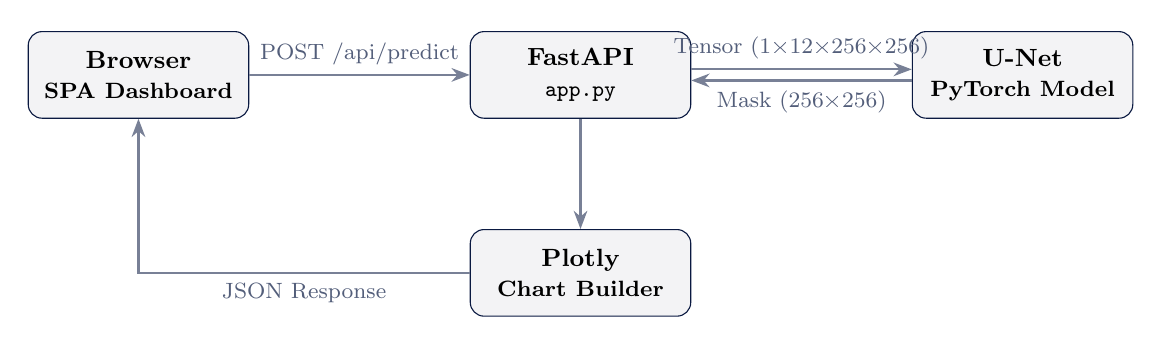
\begin{tikzpicture}[
  node distance = 1.6cm and 2.4cm,
  box/.style = {
    draw=navyblue, fill=navyblue!5, rounded corners=5pt,
    minimum width=2.8cm, minimum height=1.1cm,
    align=center, font=\small\bfseries
  },
  lbl/.style = { font=\footnotesize, midway, above, text=navyblue!70 },
  arr/.style = { -Stealth, thick, draw=navyblue!55 }
]

\node[box] (browser) {\small Browser\\\footnotesize SPA Dashboard};
\node[box, right=2.8cm of browser] (api) {\small FastAPI\\\footnotesize \texttt{app.py}};
\node[box, right=2.8cm of api]     (unet) {\small U-Net\\\footnotesize PyTorch Model};
\node[box, below=1.4cm of api]     (plotly) {\small Plotly\\\footnotesize Chart Builder};

\draw[arr] (browser.east) -- node[lbl]{POST /api/predict} (api.west);
\draw[arr] ([yshift=2pt]api.east) -- node[lbl]{Tensor (1×12×256×256)} ([yshift=2pt]unet.west);
\draw[arr] ([yshift=-2pt]unet.west) -- node[below,font=\footnotesize,text=navyblue!70]{Mask (256×256)} ([yshift=-2pt]api.east);
\draw[arr] (api.south) -- (plotly.north);
\draw[arr] (plotly.west) -| node[pos=0.25, below, font=\footnotesize, text=navyblue!70]{JSON Response} (browser.south);

\end{tikzpicture}
\end{center}

\subsection{Directory Structure}

\begin{lstlisting}[style=bash, caption={Project layout after Milestone 4}]
depi_project/
|-- models/
|   `-- best_unet_model.pth       # Trained U-Net weights
|-- src/
|   |-- model.py                  # UNet architecture class
|   |-- dataset.py                # Dataset + stratified split
|   |-- features.py               # NDVI, PCA, Mutual Info
|   |-- train.py                  # Training loop & evaluation
|   `-- utils.py                  # Plotting helpers
|-- deployment/
|   |-- app.py                    # FastAPI application
|   `-- templates/
|       `-- index.html            # Single-page web dashboard
|-- reports/
|   |-- eda_report.md
|   |-- preprocessing.md
|   `-- technical_documentation.tex   # <-- This document
|-- requirements.txt
`-- main.py                       # Full CLI pipeline runner
\end{lstlisting}

\subsection{FastAPI Backend (\texttt{deployment/app.py})}

\subsubsection{Startup: Model Loading}

The U-Net model is loaded once at server startup from the saved checkpoint and held in memory:

\begin{lstlisting}[style=python, caption={Model initialisation at startup}]
device = torch.device("cuda" if torch.cuda.is_available() else "cpu")
model  = UNet(n_channels=12, n_classes=5).to(device)

ckpt = torch.load("../models/best_unet_model.pth",
                  map_location=device, weights_only=False)
model.load_state_dict(ckpt["model_state_dict"])
model.eval()
print(f"Model ready - epoch {ckpt['epoch']}, "
      f"val mIoU {ckpt['val_miou']*100:.2f}%")
\end{lstlisting}

\subsubsection{In-Memory Preprocessing}

Each uploaded \tif{} file is processed entirely in memory — no temporary files are written to disk:

\begin{lstlisting}[style=python, caption={Preprocessing pipeline (\texttt{preprocess} function)}]
def preprocess(file_bytes: bytes) -> torch.Tensor:
    with rasterio.open(io.BytesIO(file_bytes)) as src:
        img = src.read(list(range(1, 13))).astype(np.float32)
    img = np.clip(img / 10_000.0, 0.0, 1.0)           # Normalise
    t   = torch.from_numpy(img).unsqueeze(0)
    t   = F.interpolate(t, size=(256, 256),            # Resize
                        mode="bilinear", align_corners=False)
    return t.squeeze(0)                                 # (12, 256, 256)
\end{lstlisting}

\subsubsection{API Endpoints}

\begin{center}
\renewcommand{\arraystretch}{1.25}
\begin{tabular}{lllp{6.5cm}}
\toprule
\textbf{Method} & \textbf{Path} & \textbf{Content-Type} & \textbf{Description} \\
\midrule
\texttt{GET}  & \texttt{/}            & \texttt{text/html}         & Jinja2-rendered single-page dashboard \\
\texttt{POST} & \texttt{/api/predict} & \texttt{application/json}  & Accept \tif{} upload; return prediction results and three Plotly chart specifications \\
\bottomrule
\end{tabular}
\end{center}

\subsubsection{Prediction Response Schema}

\begin{lstlisting}[style=json, caption={JSON response from \texttt{POST /api/predict}}]
{
  "filename":         "Alexandria_001_29.955_31.110.tif",
  "dominant_class":   "Desert / Bare Soil",
  "classes_detected": 4,
  "total_pixels":     65536,
  "percentages": {
    "Trees / Forest":           0.00,
    "Agriculture / Vegetation": 12.45,
    "Desert / Bare Soil":       71.32,
    "Water Bodies":              3.12,
    "Urban / Roads":            13.11
  },
  "charts": {
    "rgb":        { "data": [...], "layout": {...} },
    "prediction": { "data": [...], "layout": {...} },
    "bar":        { "data": [...], "layout": {...} }
  }
}
\end{lstlisting}

\subsubsection{Plotly Visualizations}

Three figures are generated server-side using the \texttt{plotly} Python library and serialised to JSON via \texttt{PlotlyJSONEncoder}. The browser calls \texttt{Plotly.newPlot()} with the pre-computed data, avoiding client-side data transformation.

\begin{center}
\renewcommand{\arraystretch}{1.2}
\begin{tabular}{llp{7cm}}
\toprule
\textbf{Figure} & \textbf{Plotly Type} & \textbf{Description} \\
\midrule
RGB Composite       & \texttt{px.imshow}   & 2\%--98\% percentile-stretched B04/B03/B02 mapped to R/G/B \\
Classification Map  & \texttt{go.Heatmap}  & Per-pixel class index with discrete colour scale; hover displays class name \\
Area Distribution   & \texttt{go.Bar}      & Percentage coverage per class with per-class colour coding \\
\bottomrule
\end{tabular}
\end{center}

All figures use transparent backgrounds (\texttt{paper\_bgcolor}, \texttt{plot\_bgcolor} = \texttt{"rgba(0,0,0,0)"}) to integrate with the dark dashboard theme.

\subsection{Frontend — Animated Single-Page Dashboard}

The frontend is a self-contained HTML file with zero build-step dependencies. It is served via Jinja2 templates and communicates with the backend exclusively via a single \texttt{fetch} call.

\subsubsection{Technology Stack}

\begin{center}
\renewcommand{\arraystretch}{1.2}
\begin{tabular}{lll}
\toprule
\textbf{Technology} & \textbf{Source} & \textbf{Role} \\
\midrule
Tailwind CSS v3    & CDN & Utility-class styling \\
Plotly.js v2.27    & CDN & Interactive chart rendering \\
Space Grotesk      & Google Fonts & Display / heading typography \\
Inter              & Google Fonts & Body text \\
JetBrains Mono     & Google Fonts & Data values and code labels \\
Canvas API         & Native & Animated starfield background \\
\bottomrule
\end{tabular}
\end{center}

\subsubsection{Visual Design System}

\begin{center}
\renewcommand{\arraystretch}{1.2}
\begin{tabular}{lll}
\toprule
\textbf{Token} & \textbf{Hex} & \textbf{Use} \\
\midrule
Background deep  & \texttt{\#04080f} & Page base, navbar \\
Background card  & \texttt{\#0c1526} (70\%) & Glassmorphism cards \\
Primary accent   & \texttt{\#10b981} (Emerald) & Borders, buttons, glow effects \\
Secondary accent & \texttt{\#06b6d4} (Cyan) & Satellite dot, orbit ring \\
Tertiary accent  & \texttt{\#8b5cf6} (Violet) & Inner orbit ring \\
Text primary     & \texttt{\#f1f5f9} & Headings and body \\
Text muted       & \texttt{\#94a3b8} & Labels and descriptions \\
\bottomrule
\end{tabular}
\end{center}

Glassmorphism is achieved via:
\begin{verbatim}
background: rgba(12, 21, 38, 0.80);
border: 1px solid rgba(148, 163, 184, 0.07);
backdrop-filter: blur(24px);
\end{verbatim}

\subsubsection{Animated Components}

\begin{enumerate}[leftmargin=*, label=\textbf{\arabic*.}]
  \item \textbf{Starfield Canvas:} 200 twinkling stars rendered via \texttt{requestAnimationFrame} on a fixed \texttt{<canvas>} element behind all page content. Each star has an independent sinusoidal opacity cycle.

  \item \textbf{Satellite Orbit Animation:} A carrier \texttt{<div>} sized to match the orbit track rotates via \texttt{animation: orbitSpin 18s linear infinite}. The satellite SVG icon is positioned at the top of the carrier and applies a counter-rotation \texttt{animation: counterSpin18} to remain upright as it orbits:
  \[
    \text{Carrier rotation} + \text{Counter-rotation} = \text{Net: translates along circle, no spinning}
  \]

  \item \textbf{Drag-and-Drop Upload Zone:} Native browser drag events (\texttt{dragover}, \texttt{dragleave}, \texttt{drop}) toggle a CSS class \texttt{.over} that adds an emerald border glow and a radial gradient background.

  \item \textbf{Animated Progress Steps:} Four processing steps are displayed in sequence while the API call runs. Critically, the step animation and the \texttt{fetch} call are executed in \textbf{parallel} via \texttt{Promise.all([apiCall, stepAnim])}, so the animation adds \textbf{zero} latency to total processing time. Each step transitions from inactive → active (spinner) → done (green checkmark).

  \item \textbf{Results Dashboard:} Sections fade in with \texttt{opacity} transitions. Legend cards animate in with staggered \texttt{animation-delay}. Percentage fill bars animate from \texttt{width: 0\%} to their final value via a CSS transition with cubic-bezier easing.
\end{enumerate}

\subsubsection{User Journey}

\begin{center}
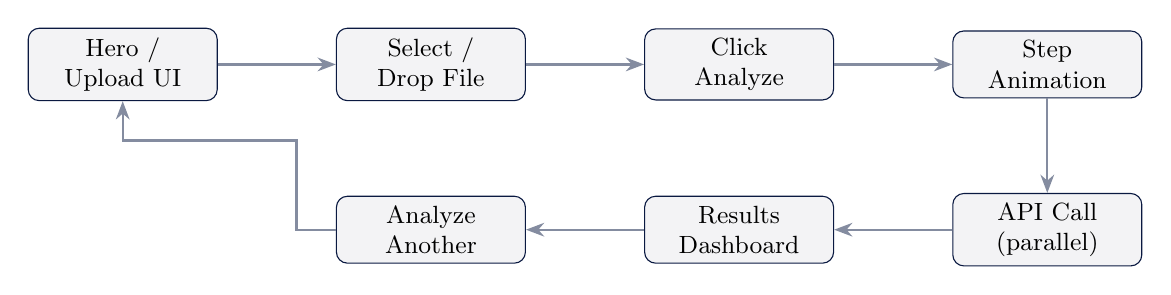
\begin{tikzpicture}[
  node distance = 0.9cm and 1.5cm,
  st/.style = {
    draw=navyblue, fill=navyblue!5, rounded corners=4pt,
    minimum width=2.4cm, minimum height=0.85cm,
    align=center, font=\small
  },
  arr/.style = { -Stealth, thick, draw=navyblue!50 }
]

\node[st] (A) {Hero /\\Upload UI};
\node[st, right=1.5cm of A] (B) {Select /\\Drop File};
\node[st, right=1.5cm of B] (C) {Click\\Analyze};
\node[st, right=1.5cm of C] (D) {Step\\Animation};
\node[st, below=1.2cm of D] (E) {API Call\\(parallel)};
\node[st, left=1.5cm of E]  (F) {Results\\Dashboard};
\node[st, left=1.5cm of F]  (G) {Analyze\\Another};

\draw[arr] (A) -- (B);
\draw[arr] (B) -- (C);
\draw[arr] (C) -- (D);
\draw[arr] (D) -- (E);
\draw[arr] (E) -- (F);
\draw[arr] (F) -- (G);
\draw[arr] (G.west) -- ++(-0.5,0) |- ([yshift=-0.5cm]A.south) -- (A.south);

\end{tikzpicture}
\end{center}

\subsection{Starting the Application}

\begin{lstlisting}[style=bash, caption={Installation and startup}]
# Step 1: Install all dependencies
pip install -r requirements.txt

# Step 2: Start the FastAPI server
cd depi_project/deployment
python app.py

# Server prints:
#   Model loaded -- epoch N, val mIoU XX.XX%
#   Uvicorn running on http://0.0.0.0:8000

# Step 3: Open the dashboard
# Navigate to: http://localhost:8000
# Upload any .tif from egypt_s2_diverse_dataset/
\end{lstlisting}

% ============================================================
\section{Dependency Reference}
% ============================================================

\begin{center}
\renewcommand{\arraystretch}{1.25}
\begin{tabular}{lll}
\toprule
\textbf{Package} & \textbf{Primary Role} & \textbf{Pipeline Stage} \\
\midrule
\texttt{torch}            & Deep learning framework       & Training, inference \\
\texttt{torchvision}      & Image transformation utilities & Training \\
\texttt{rasterio}         & GeoTIFF I/O                   & All stages \\
\texttt{numpy}            & Numerical computation          & All stages \\
\texttt{scikit-learn}     & PCA, mutual information        & Feature engineering \\
\texttt{matplotlib}       & Static figure generation       & EDA, training curves \\
\texttt{fastapi}          & REST API framework             & Deployment \\
\texttt{uvicorn}          & ASGI web server                & Deployment \\
\texttt{python-multipart} & Multipart file upload parsing  & Deployment \\
\texttt{jinja2}           & HTML template rendering        & Deployment \\
\texttt{plotly}           & Interactive visualizations     & Deployment \\
\bottomrule
\end{tabular}
\end{center}

% ============================================================
\section{Key Design Decisions}
% ============================================================

\begin{enumerate}[leftmargin=*, label=\textbf{\arabic*.}, itemsep=6pt]
  \item \textbf{FastAPI over Flask.}
    FastAPI provides native \texttt{async}/\texttt{await} I/O, automatic OpenAPI documentation at \texttt{/docs}, and request/response type validation via Pydantic — all at essentially the same development complexity as Flask. The async foundation is particularly important for production readiness, where concurrent inference requests should not block each other on I/O.

  \item \textbf{Server-side Plotly serialisation.}
    Plotly figures are fully constructed in Python (where the NumPy arrays already reside post-inference) and serialised to JSON once. The browser receives a static JSON specification and renders it — eliminating any JavaScript data transformation and keeping the frontend dependency-free beyond Plotly.js.

  \item \textbf{Parallel animation and API call.}
    Step animation and the \texttt{fetch} call run concurrently via \texttt{Promise.all}. This ensures the animated pipeline steps provide a visual progress indicator with \textit{zero added latency}: if inference completes before the animation finishes, results display immediately after the final step.

  \item \textbf{Inverse-frequency loss weighting.}
    Oversampling rare classes (e.g.\ Trees/Forest at 0.61\%) would inflate the training dataset by a factor of $\sim$85 for that class, dramatically increasing training time. Loss weighting achieves equivalent gradient correction at zero additional compute cost.

  \item \textbf{Stratified geographic splitting.}
    Splitting randomly without stratification risks placing all tiles from a narrow-coverage class (e.g.\ water tiles predominant only in PhilaeAswan) entirely in training, leading to optimistic validation metrics. Stratification by region prefix ensures representative class coverage in all three subsets.

  \item \textbf{In-memory file processing.}
    The API reads the uploaded \tif{} into a \texttt{bytes} buffer and passes it directly to \texttt{rasterio.open(io.BytesIO(...))} — no temporary files are written to disk. This improves security, simplifies deployment in containerised environments, and eliminates file cleanup concerns.
\end{enumerate}

% ============================================================
\section{Conclusion}
% ============================================================

SentinelVision delivers a complete, end-to-end remote sensing analysis pipeline: from raw 12-band \sentinel{} GeoTIFF data through U-Net semantic segmentation to an animated, real-time web dashboard. The system achieves all requirements of DEPI Milestone 4 and provides a modular, production-ready codebase.

The clean separation between the \texttt{src/} research layer and the \texttt{deployment/} serving layer means the trained model can be updated (by rerunning \texttt{main.py}) without any changes to the API or frontend. The FastAPI backend and glassmorphism dashboard collectively deliver a presentation layer appropriate for both technical and non-technical stakeholders.

\begin{keybox}[Potential Extensions]
\begin{itemize}[leftmargin=*, noitemsep]
  \item \textbf{Additional spectral indices:} NDWI (water), NDBI (built-up area), SAVI (soil-adjusted vegetation) as engineered input features
  \item \textbf{Change detection mode:} upload two tiles from different acquisition dates; overlay predicted masks to quantify land cover transitions
  \item \textbf{GeoTIFF export:} return the prediction mask as a georeferenced \tif{} with embedded CRS metadata, ready for GIS analysis
  \item \textbf{Cloud deployment:} Docker containerisation + GPU-backed cloud instance (AWS EC2 / GCP Compute Engine) for production throughput
  \item \textbf{Larger backbone:} replace the standard U-Net encoder with a pretrained ResNet-50 or EfficientNet backbone via transfer learning
\end{itemize}
\end{keybox}

% ============================================================
%  References
% ============================================================
\newpage
\begin{thebibliography}{9}

\bibitem{ronneberger2015}
O.~Ronneberger, P.~Fischer, and T.~Brox,
``U-Net: Convolutional Networks for Biomedical Image Segmentation,''
in \textit{Proc. MICCAI}, 2015.
\url{https://arxiv.org/abs/1505.04597}

\bibitem{esa2024}
European Space Agency,
\textit{Sentinel-2 Mission Guide},
ESA, 2024.
\url{https://sentinel.esa.int/web/sentinel/missions/sentinel-2}

\bibitem{loshchilov2019}
I.~Loshchilov and F.~Hutter,
``Decoupled Weight Decay Regularization,''
in \textit{Proc. ICLR}, 2019.
\url{https://arxiv.org/abs/1711.05101}

\bibitem{riquelme2021}
J.~A.~Riquelme, R.~Tapia, and A.~Garrido,
``Land Cover Classification Using Sentinel-2 Imagery and Deep Learning,''
\textit{Remote Sensing}, vol.~13, no.~1, 2021.

\bibitem{fastapi}
S.~Ram\'{i}rez,
\textit{FastAPI Documentation},
2024.
\url{https://fastapi.tiangolo.com/}

\bibitem{plotly}
Plotly Technologies Inc.,
\textit{Collaborative data science},
2024.
\url{https://plotly.com}

\end{thebibliography}

\end{document}
